\begin{frame}{Modélisation}
    \begin{center}
        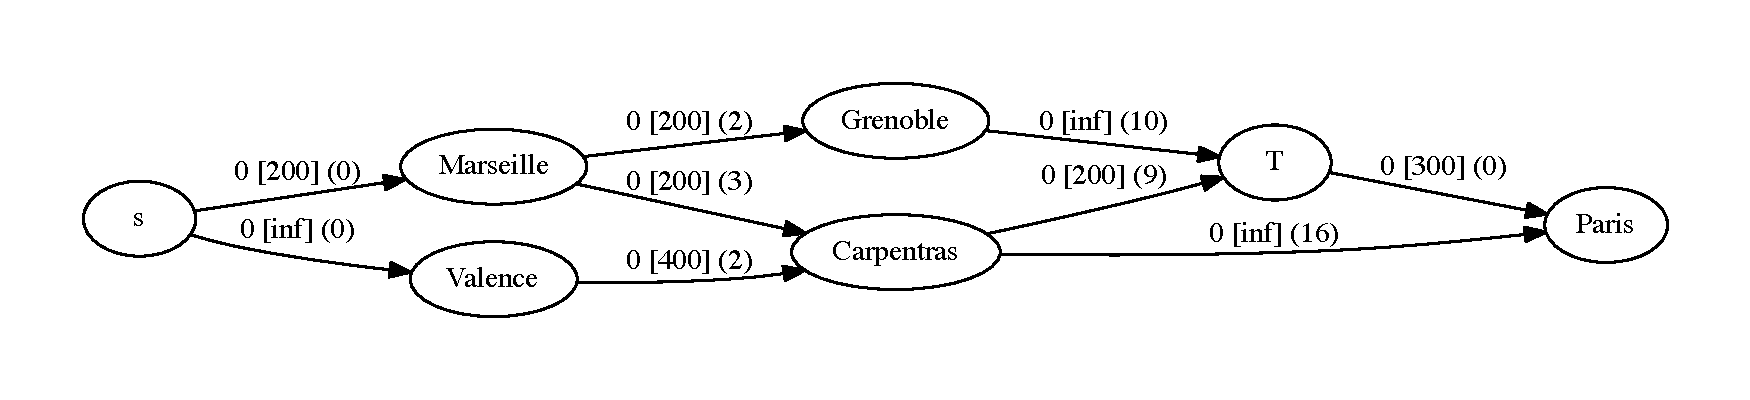
\includegraphics[width=\textwidth]{tutorials/flmcmin/fleurs-1.pdf}
    \end{center}
    Idée : train = 1 sommet supplémentaire
\end{frame}

\begin{frame}{Simplification}
    \begin{center}
        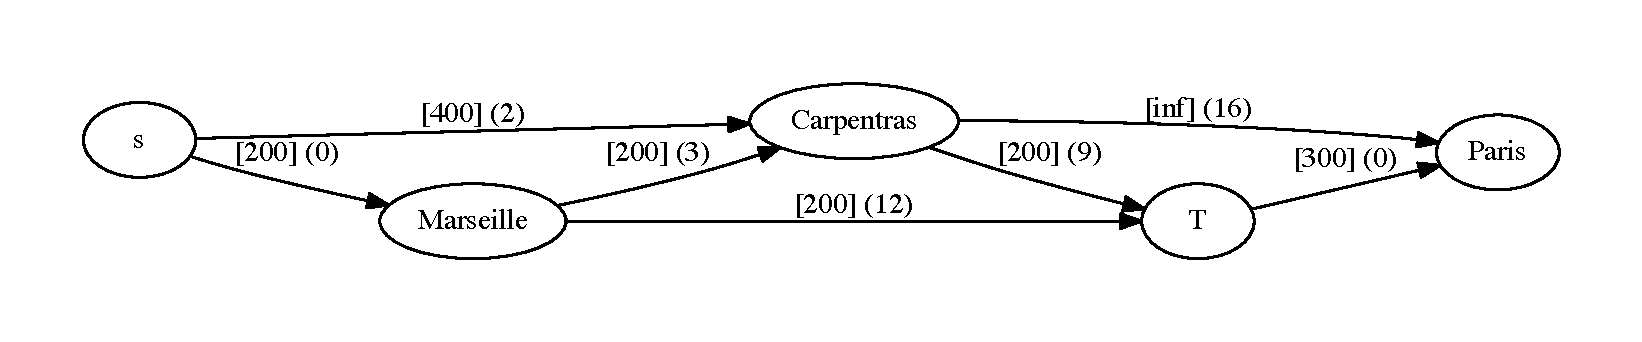
\includegraphics[width=\textwidth]{tutorials/flmcmin/fleurs-2.pdf}
    \end{center}
    Suppression des sommets Grenoble et Valence (loi de conservation)
\end{frame}



\begin{frame}{Résolution}
    Plus court chemin : s-Carpentras-T-Paris pour un coût de 11. On peut augmenter le flot de 200
    \begin{center}
        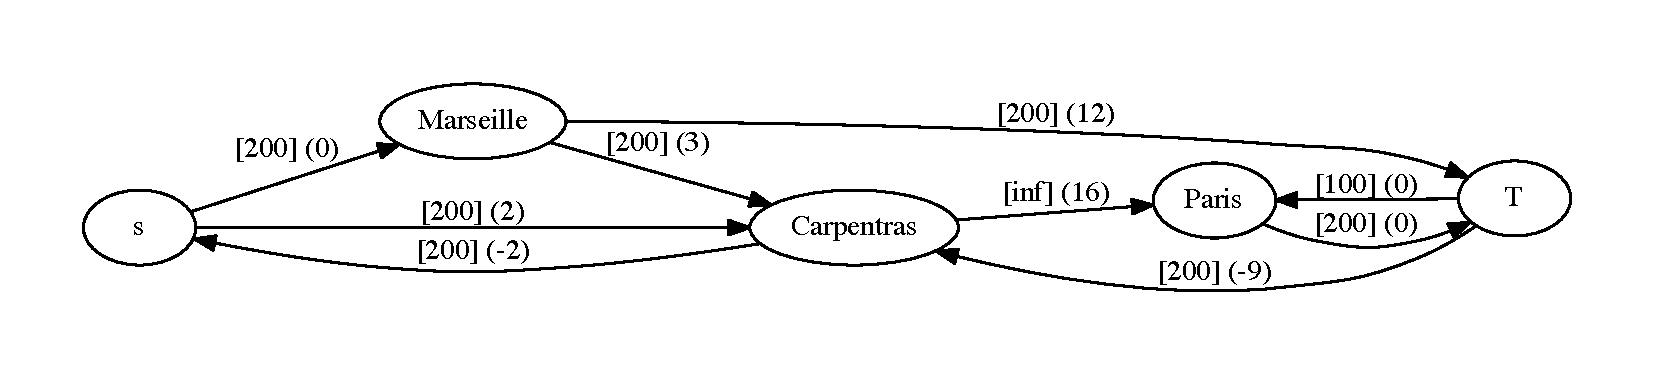
\includegraphics[width=\textwidth]{tutorials/flmcmin/fleurs-3.pdf}
    \end{center}
\end{frame}

\begin{frame}{Résolution}
    Plus court chemin : s-Marseille-T-Paris pour un coût de 12 et augmenter le flot de 100 à nouveau
    \begin{center}
        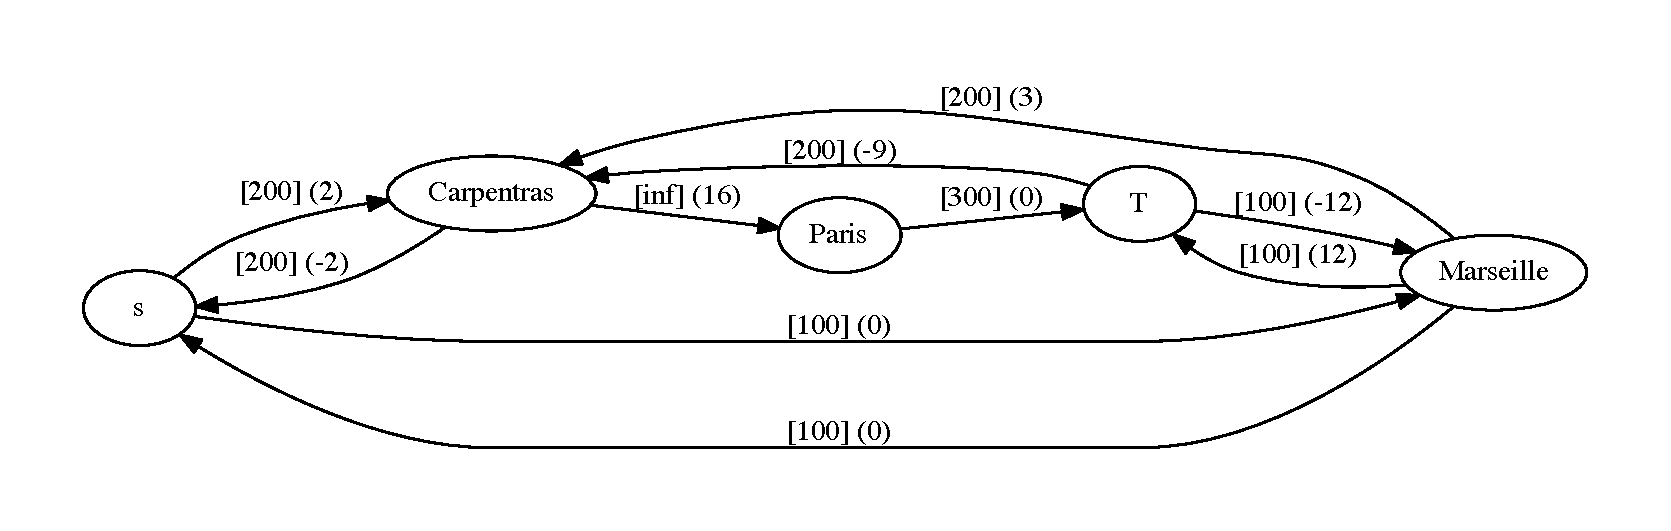
\includegraphics[width=\textwidth]{tutorials/flmcmin/fleurs-4.pdf}
    \end{center}
\end{frame}

\begin{frame}{Résolution}
    Plus court chemin : s-Carpentras-Paris qui a un coût de 18 et permet d'augmenter le flot de 200
    \begin{center}
        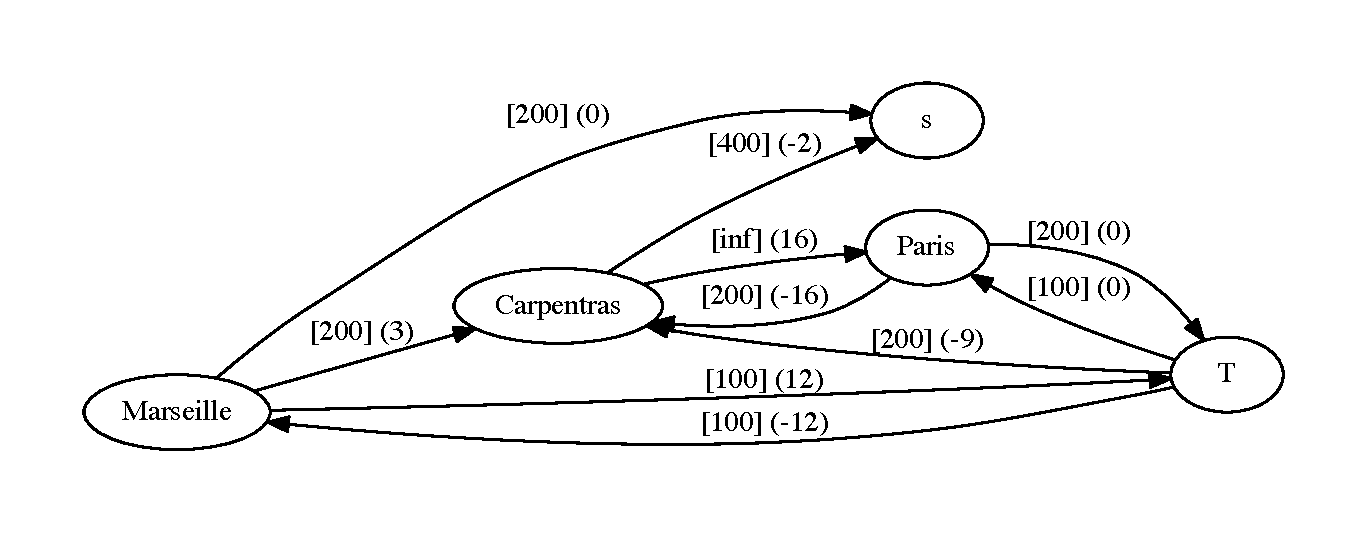
\includegraphics[width=\textwidth]{tutorials/flmcmin/fleurs-5.pdf}
    \end{center}
\end{frame}

\begin{frame}{Résolution}
    Dernier chemin possible : s-Marseille-Carpentras-Paris pour un coût de 19 et une augmentation de flot de 100.
    \begin{center}
        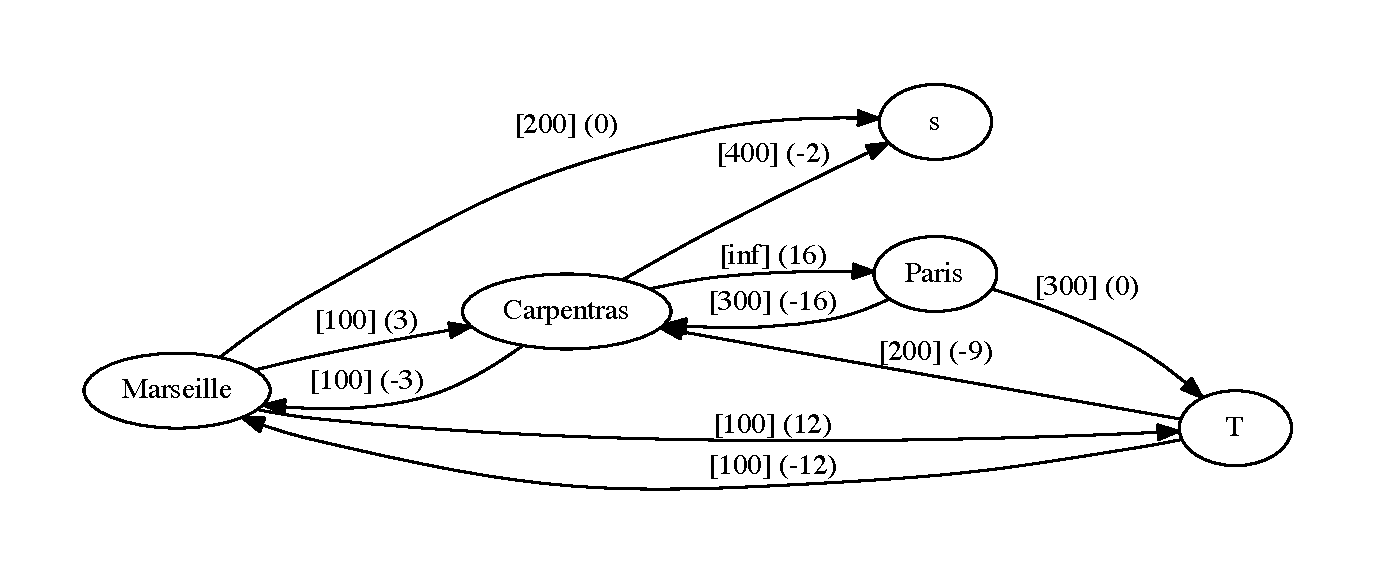
\includegraphics[width=\textwidth]{tutorials/flmcmin/fleurs-6.pdf}
    \end{center}
\end{frame}
